% !TeX root = ../../progress-sem1.tex
% Section: AI pipeline development, matching "การพัฒนา AI pipeline" in the example.
% Input from chapters/03-methodology.tex, before "การพัฒนาระบบ".

\section{การพัฒนา AI pipeline}\label{sec:ai-pipeline}
\thaijustify{
  AI ในแพลตฟอร์มทำงานสี่ส่วน ได้แก่ การร่าง user story การร่าง structured prompt การสร้าง UI variant และการวิเคราะห์ข้อเสนอแนะของผู้เข้าร่วมทดสอบ ในภาคการศึกษาที่ 1 ทีมพัฒนาสามส่วนแรกจนใช้งานผ่านหน้าจอได้ และพัฒนาส่วนการวิเคราะห์ข้อเสนอแนะไว้ที่ backend
}

\subsection{วิเคราะห์ความต้องการของระบบที่ใช้ AI}
\thaijustify{
  ผลลัพธ์ของ AI ต้องนำไปใช้ต่อในระบบได้ทันที จึงกำหนดให้โมเดลตอบเป็น JSON ตาม schema (structured output) และ UI ที่สร้างต้องเป็น HTML ที่ใช้ component ของ UI kit ที่นักออกแบบเลือก ใช้สีแบรนด์ตาม design intent และผ่านมาตรฐานการเข้าถึงที่กำหนด นอกจากนี้งานแต่ละชิ้นใช้เวลาหลายนาที ระบบจึงต้องแสดงความคืบหน้าแบบ real-time และให้ผู้ใช้ยกเลิกงานได้
}

\subsection{การเลือกโมเดลและบริการ AI}
\thaijustify{
  ระบบเรียกโมเดลผ่าน CPE AI Gateway ของภาควิชา ซึ่งให้บริการ API แบบเดียวกับ OpenAI จึงเปลี่ยนโมเดลได้ด้วยการตั้งค่า โดยไม่ต้องแก้โค้ด โมเดลที่ใช้ ได้แก่ muse-glimmer-30b สำหรับสร้าง UI และ qwen3.8-27b สำหรับงานที่ต้องการ structured output เช่น การร่าง prompt, user story, persona และการวิเคราะห์ข้อเสนอแนะ ระบบเปิดขั้นการคิด (reasoning) ของโมเดลไว้เป็นค่าเริ่มต้น เพื่อแสดงความคิดของโมเดลใน generation trace
  ทีมเลือกใช้โมเดลทั้งสองเนื่องจากเป็นโมเดลที่ภาควิชาเปิดให้ใช้ได้โดยไม่มีค่าใช้จ่าย จึงเหมาะกับช่วงพัฒนาที่ต้องเรียกโมเดลซ้ำหลายครั้ง
}

\subsection{การร่าง Structured Prompt}
\thaijustify{
  เมื่อนักออกแบบเลือก user story ระบบรวม design intent, persona และ user story เป็น context แล้วให้โมเดลร่าง structured prompt งานนี้รันเป็น background job บน BullMQ หน้าจอจึงกลับมาเชื่อมต่อกับงานเดิมผ่าน SSE ได้หากผู้ใช้ออกจากหน้าแล้วกลับมา ระบบแสดงจำนวน token ระหว่างร่าง และไม่บันทึกความคิดดิบของโมเดลลงฐานข้อมูล
}

\subsection{การสร้าง UI Variant พร้อมการตรวจและแก้ไขอัตโนมัติ}
\thaijustify{
  การสร้าง UI เป็นไปตามขั้นตอนในรูปที่~\ref{fig:generation-pipeline} ระบบสร้าง persona artifact จาก prompt ก่อน (ข้ามขั้นนี้ได้หากนักออกแบบเลือก persona ไว้แล้ว) จากนั้นสร้างหน้าจอแบบ high-fidelity เป็น HTML ทีละ variant ค่าเริ่มต้นคือสอง variant (A และ B) สำหรับ comparative usability testing HTML ที่ได้จะถูก sanitize และตรวจโครงสร้าง การใช้ component ของ UI kit สีแบรนด์ platform และการเข้าถึงตามมาตรฐานใน design intent หากไม่ผ่าน ระบบส่งปัญหาที่พบกลับให้โมเดลแก้ได้สูงสุดสองครั้ง และหากยังไม่ผ่านจะเริ่มสร้าง variant นั้นใหม่อีกหนึ่งครั้งโดยแจ้งโมเดลว่าครั้งก่อนผิดพลาดตรงไหน
}
\begin{figure}[H]
  \centering
  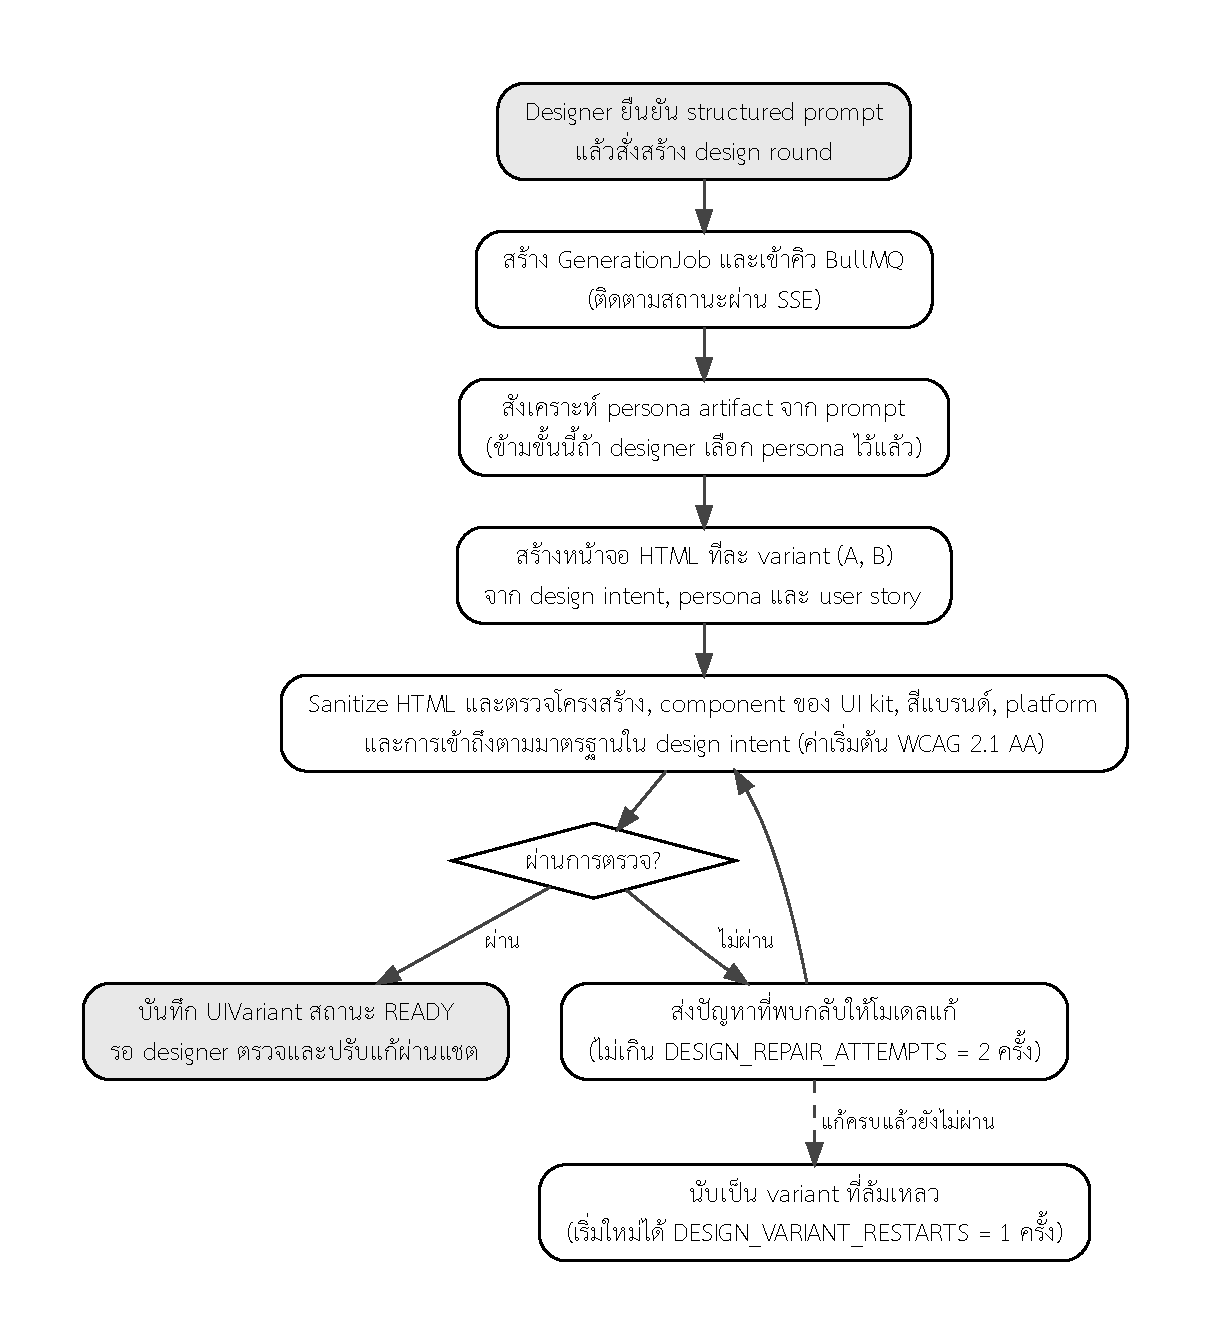
\includegraphics[width=0.78\linewidth]{figures/ch3-methodology/generation-pipeline.pdf}
  \caption{ขั้นตอนการสร้าง UI variant ด้วย AI}
  \label{fig:generation-pipeline}
\end{figure}

\subsection{Generation Trace}
\thaijustify{
  ระหว่างสร้าง UI หน้าจอแสดงความคิดของโมเดลและสถานะของแต่ละขั้นแบบ real-time ผ่าน SSE พร้อมเวลาที่ใช้จริงและผลการตรวจจริงของแต่ละ variant รอบการแก้ไขภายในจะไม่แสดงให้ผู้ใช้เห็น เพื่อให้ trace อ่านง่าย และหาก backend เริ่มสร้าง variant ใหม่ trace จะติดตามงานใหม่ต่อโดยอัตโนมัติ
  \todo{ภาพหน้าจอ generation trace}
}

\subsection{การวิเคราะห์ข้อเสนอแนะของผู้ใช้ (Backend)}
\thaijustify{
  backend รองรับการให้โมเดลวิเคราะห์ข้อเสนอแนะและพฤติกรรมของผู้เข้าร่วมทดสอบ แล้วจัดกลุ่มเป็นประเด็น (theme) ให้นักออกแบบเลือกไปเริ่มรอบการออกแบบถัดไป ข้อมูลส่วนบุคคลถูกลบออกก่อนส่งให้โมเดล หน้าจอของส่วนนี้อยู่ในแผนของภาคการศึกษาที่ 2
  \todo{ชุดข้อมูลและผลการประเมินคุณภาพผลลัพธ์ของ AI}
}
